% -*-LaTeX-*-

% $Log: convolution.tex,v $
% Revision 1.6  2007/12/11 02:32:54  stiber
% Small edits for start of Winter 2008.
%
% Revision 1.5  2007/03/20 23:53:12  stiber
% Updated LaTeX.
%
% Revision 1.4  2007/03/20 01:25:56  stiber
% Modifications made to make this a standalone text.
%
% Revision 1.3  2006/03/27 23:36:42  stiber
% Fixed error in formula.
%
% Revision 1.2  2004/03/29 19:51:48  stiber
% Updated for Spring 2004 and new textbook (DSP First).
%
% Revision 1.1  2004/02/19 00:26:01  stiber
% Initial revision
%

\chapter{The Z-Transform and Convolution}
\label{ch:convolution}

Two signal processing tools --- the \emph{z transform} and
\emph{convolution} --- are introduced in this chapter.  These
operations play important roles in the analysis of discrete-time
signals (which is what we do in the computer). We shall see that they
are related --- the convolution of two time-domain signals (which is
what we do when we filter a signal) is equivalent to multiplication of
their corresponding z-transforms. This is one example of how these
representations can greatly simplify computation.

After studying this chapter, you should be able to understand what the
z-transform and convolution are, and how to implement them. You should
understand the differences between them and the other transforms:
Fourier series, Fourier transform, and discrete Fourier transform. You
will enrich your knowledge of filter transfer functions with its time
domain representation: its \emph{impulse response}.

\section{Domains}

Up to this point, we have covered the Fourier series representation of
a signal as a weighted sum of sinusoids. In effect, the Fourier series
\emph{transforms} a finite and periodic, continuous signal in the time
\emph{domain} into an infinite, discrete spectrum in the frequency
\emph{domain}.
\index{domains}
\index{time domain}
\index{frequency domain}
\index{domain!time}
\index{domain!frequency}
When we use the term \emph{domain}, we merely mean a particular way of
looking at a signal. In this case, we have two different ways of
thinking about our signals: as functions of time or as functions of
frequency. These are equivalent, in the sense that we can convert the
signal's representation back and forth between the two domains without
loss of information (neglecting matters such as roundoff error).

In future chapters, we will cover two other transforms:
\begin{description}
\item[Fourier transform] transforms an infinite, continuous signal in
the time domain into an infinite, continuous spectrum in the frequency
domain.

\item[Discrete Fourier transform] transforms a finite, discrete signal
in the time domain into a finite, discrete spectrum in the frequency
domain.
\end{description}

Here, however, we will learn about the
\emph{z-transform}, which converts an infinite, discrete signal in the
time domain into a finite, continuous spectrum in the frequency
domain. The z-transform fills the last combination among ``finite vs.
infinite; continuous vs. discrete''. Table~\ref{tb:zt-transforms}
summarizes all four transforms.  As you can see, continuous versus
discrete in the time domain transforms to infinite versus finite in
the frequency domain, while finite versus infinite in the time domain
transforms to discrete versus continuous in the frequency domain.

\begin{table}
\caption{Summary of frequency transforms.
\label{tb:zt-transforms}}
\begin{center}
\begin{tabular}{|l|l|l|} \hline
Transform & Time Domain & Frequency Domain\\ \hline\hline
Fourier Series & Finite, Continuous & Infinite, Discrete \\ 
Fourier Transform & Infinite, Continuous & Infinite, Continuous \\ 
Discrete Fourier Transform & Finite, Discrete & Finite, Discrete \\ 
Z-Transform & Infinite, Discrete & Finite, Continuous \\ \hline
\end{tabular}
\end{center}
\end{table}

\section{The z-transform}
The \emph{z-transform} of a discrete time signal $x[n]$, $n=0, \pm 1,
\pm 2, \ldots, \pm\infty$ is defined as the power series
\begin{equation}
X(z) \equiv \sum_{k=-\infty}^{\infty} x[k] z^{-k}
\label{eq:zt}
\end{equation}
where $z$ is a continuous complex variable. It transforms the time
domain, infinite, discrete sequence into its complex plane
representation $X(z)$. Since the z-transform is an infinite power
series, it exists only for those values of $z$ for which this series
converges. The \emph{region of convergence} (ROC) of $X(z)$ is the set
of all values of $z$ for which $X(z)$ has a finite value. We consider
the z-transform to be a transform between the time domain and the
frequency domain because we can substitute $z=e^{j\hat{\omega}}$ into
equation~(\ref{eq:zt}) to get the signal's (finite and continuous)
frequency content $\mathcal{X}(\hat{\omega})$ --- just as we
previously made the same substitution to derive a feedforward filter's
frequency response from its transfer function.

The relationship between $x[n]$ and $X(z)$ can be indicated
by the \emph{transform pair}
\begin{equation}
\underbrace{x[n]}_{\stackrel{\text{function of}}{_\text{sample \#}}}
   \stackrel{\mathbf{Z}}{\longleftrightarrow} 
   \underbrace{X(z)}_{\stackrel{\text{function of}}{_\text{complex $z$}}}
\end{equation}

\problemset{
\subsubsection{Self-Test Exercises}

See~\ref{sc:ch6ex} \#\ref{it:ch6ex1}--\ref{it:ch6ex2} for answers.

\begin{enumerate}
\item Determine the z-transform for the sequence
  $x[n]=\{1,2,5,7,0,1\}$, $n=0,1,2,3,4,5$

\item Determine the z-transform of the sequence
  $x[n]=\{1,2,5,7,0,1\}$, $n=-2,-1,0,1,2,3$
\end{enumerate}}

\subsection{Example: z-transform of an impulse}

\index{z-transform!of an impulse}
\index{unit impulse}
The \emph{unit impulse} or \emph{unit sample} signal is the $\delta$
function,
\begin{equation}
\delta[n] = \left\{\begin{array}{ll}
                        1 & n=0 \\
                        0 & n \neq 0
          \end{array}\right.
\end{equation}
It has value of zero for every sample except $n=0$, for which it has a
value of one. Substituting this signal into~(\ref{eq:zt}) to get its
z-transform, we have
\begin{align}
\Delta(z) &= \sum_{k=-\infty}^{\infty} \delta[k] z^{-k} \notag\\
     &= 1z^{-0}=1
\end{align}
that is 
\begin{equation}
\delta[n]\stackrel{\mathbf{Z}}{\longleftrightarrow} 1
\end{equation}

Since the frequency content of the signal is the magnitude of its
z-transform on the unit circle in the z-plane, 
\begin{equation}
|\mathcal{D}(\hat{\omega})|=|\Delta(e^{j\hat{\omega}})|=1
\label{eq:zt-delta}
\end{equation}
This tells us that the frequency content is the same for all
frequencies: an impulse has a \emph{flat spectrum}.

What about time shifted impulses,
\begin{align}
\delta[n-n_0] &= \left\{\begin{array}{ll}
                        1 & n=n_0 \\
                        0 & n \neq n_0
          \end{array}\right., \quad n_0>0 \\
\delta[n+n_0] &= \left\{\begin{array}{ll}
                        1 & n=-n_0 \\
                        0 & n \neq -n_0
          \end{array}\right., \quad n_0>0
\end{align}
In these cases the nonzero value is not at sample zero, but at samples
$n_0$ or $-n_0$.  We can compute the z-transform as before,
\begin{align}
\Delta(z) &= \sum_{k=-\infty}^{\infty} \delta[k-n_0] z^{-k} \notag\\
          &= 1z^{-n_0}=z^{-n_0}=\frac{1}{z^{n_0}}
\end{align}
for $\delta[n-n_0]$.  The z-transform for this shifted unit impulse
has one value, $z^{-n_0}$, for any $z \neq 0$.
\begin{equation}
\delta[n-n_0] \stackrel{\mathbf{Z}}{\longleftrightarrow} \frac{1}{z^{n_0}},
\quad n_0>0
\end{equation}

Its frequency content is also one, just like $\delta[n]$ (remember
that we compute the spectrum for values of $z$ on the unit circle),
\begin{equation}
|\mathcal{D}(\hat{\omega})|=|\Delta(e^{j\hat{\omega}})|=|e^{-jn_0\hat{\omega}}|=1
\end{equation}
This is not surprising at all, because it is, after all, just a
time-shifted version of $\delta[n]$. The signal $\delta[n+n_0]$ is
left as a self-test exercise.

\problemset{
\subsubsection{Self-Test Exercises}

See~\ref{sc:ch6ex} \#\ref{it:ch6ex3}--\ref{it:ch6ex4} for answers.

\begin{enumerate}
\item Sketch equation~(\ref{eq:zt-delta}).
\item Compute the z-transform and frequency content for the signal
  $\delta[n+n_0]$.
\end{enumerate}}

\subsection{Example: z-transform of exponential signal}

\index{z-transform!of an exponential}
An exponential signal is defined as 
\begin{equation}
x[n] = \left\{\begin{array}{ll}
                        \alpha^n & \quad  n \ge 0 \\
                        0        & \quad n < 0
          \end{array}\right.
\label{eq:zt-expof}
\end{equation}
where $\alpha$ can be any real or complex value less than one. The
signal consists of an infinite number of samples. The z-transform of
this signal is
\begin{align}
X(z) &= \sum_{k=-\infty}^{\infty} x[k] z^{-k} \notag\\
     &= \sum_{k=0}^{\infty}\alpha^k  z^{-k} \notag\\
     &= \sum_{k=0}^{\infty}(\alpha z^{-1})^k
\label{eq:exp-zt}
\end{align}

This is an infinite \emph{geometric series}: a sum in which each
successive term is the previous term times some (unchanging)
expression (i.e., the ratio of successive terms is constant).
\index{geometric series} The ratio of two successive terms in a
geometric series like \index{geometric series!common ratio}
equation~(\ref{eq:exp-zt}) is called its \emph{common ratio}, which in
this case is $\alpha z^{-1}$. We can show this by rewriting
equation~(\ref{eq:exp-zt}) as $X(z) = 1 + \alpha z^{-1} + \alpha^{2}
z^{-2} + \cdots$. Rewriting the \spscript{$i+1$}{st} element of this
series as a recurrence relation (in terms of the \spscript{$i$}{th}),
we get $X(z)_{i+1} = X(z)_i \alpha z^{-1}$, which shows the common ratio.
  
If we have a geometric series in which successive terms $b_i$ and
$b_{i+1}$ have the common ratio $r$ (i.e., $b_{i+1}/b_i = r$), then
any term in the series can be expressed in terms of the first term as
\index{geometric series!as function of first term}
\begin{equation*}
b_i = b_0 r^i
\end{equation*}
So, a geometric series can be expressed as a sum of these, $b_0 + b_0r
+ b_0r^2 + \cdots$. We can factor out the zeroth term, leaving us with
the task of simplifying $1 + r + r^2 + \cdots$. Multiplying this sum
by $(1-r)/(1-r)$, we obtain
\begin{align}
(1 + r + r^2 + \cdots)\frac{1-r}{1-r}
  & = \frac{1 + r + \cdots - r - r^2 - \cdots}{1-r} \notag\\
  & = \frac{1-r^N}{1-r}
\end{align}

In this case, $|r|<1$ so $r^N \rightarrow 0$ as $N \rightarrow \infty$:
\begin{equation}
1+r+r^2+r^3+\ldots = \frac{1}{1-r}, \quad\text{if } |r|<1
\end{equation}
Consequently, for $|r|=|\alpha z^{-1}|<1$ or $|z|>|\alpha|$,
$X(z)$ converges to
\begin{equation}
X(z)=\frac{1}{1-\alpha z^{-1}}, \quad |z|>|\alpha|
\label{eq:zt-expoF}
\end{equation}

In the z-plane, $|z|>|\alpha|$ refers to any $z$ that is outside of
the radius $|\alpha|$ circle. We see that in this case, the
z-transform provides a compact alternative representation of the
signal $x[n]$.

Let's check out some special cases:

\begin{figure}
\centerline{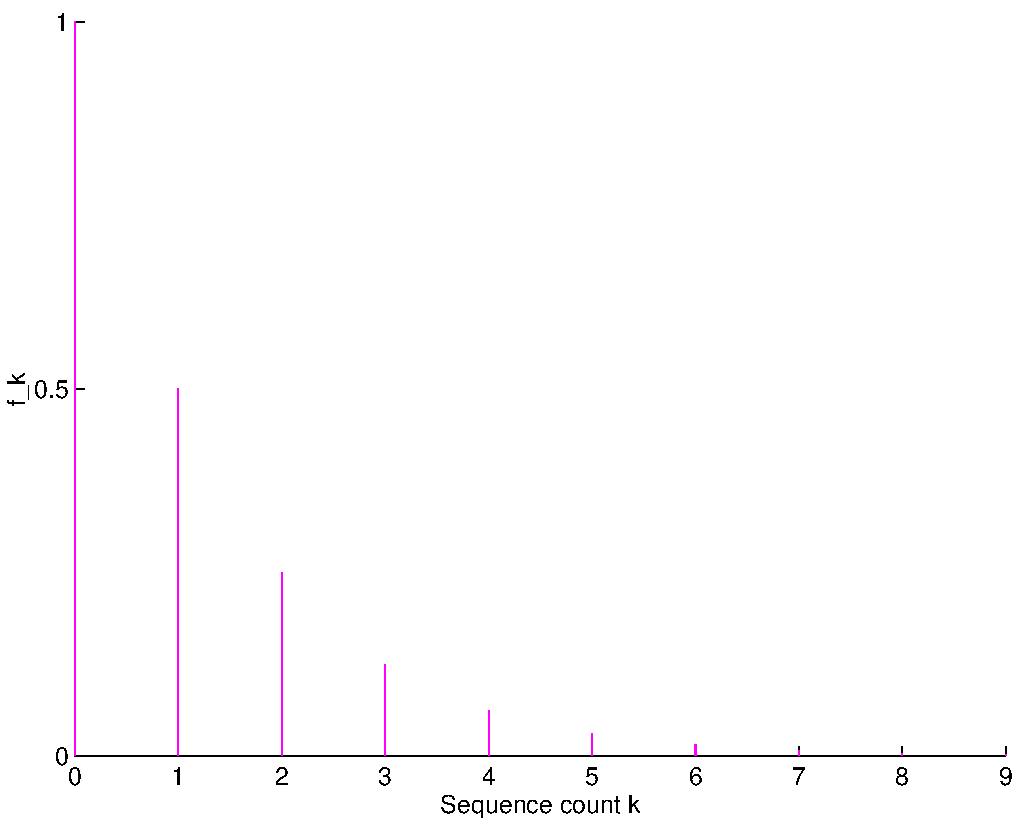
\includegraphics[width=3.5in]{ch-conv/zt_expo_rf}}
\caption{The exponential signal $x[n]=(1/2)^n, n=0,1,2,\ldots$.
\label{fig:zt-expo-r0.5f}}
\end{figure}

\paragraph*{When $\alpha$ is a real number, say $\alpha=1/2$:}
The discrete signal in this case is 
\begin{equation}
x[n] = \left\{\begin{array}{ll}
                        \left(\frac{1}{2}\right)^n & \quad  n \ge 0 \\
                        0             & \quad n < 0
          \end{array}\right.
\end{equation}
or
\begin{equation}
x[n] = \left\{1, \frac{1}{2}, \left(\frac{1}{2}\right)^2,
        \left(\frac{1}{2}\right)^3, \ldots, \right\}
\end{equation}
Figure~\ref{fig:zt-expo-r0.5f} shows the graph of the signal $x[n]$.

Replacing $\alpha$ with $1/2$ in~(\ref{eq:zt-expoF}), its
z-transform is expressed as
\begin{equation}
X(z)=\frac{1}{1-\frac{1}{2}z^{-1}}, \quad |z|>\frac{1}{2}
\end{equation}

As you should be familiar with now, the frequency content of this
signal is the magnitude of its z-transform on the unit circle
$z=e^{j\hat{\omega}}$ in the z-plane, which is
\begin{equation}
|\mathcal{X}(\hat{\omega})|=|X(e^{j\hat{\omega}})|
           =\left|\frac{1}{1-\frac{1}{2}e^{-j\hat{\omega}}}\right|
\end{equation}

\begin{figure}
\centerline{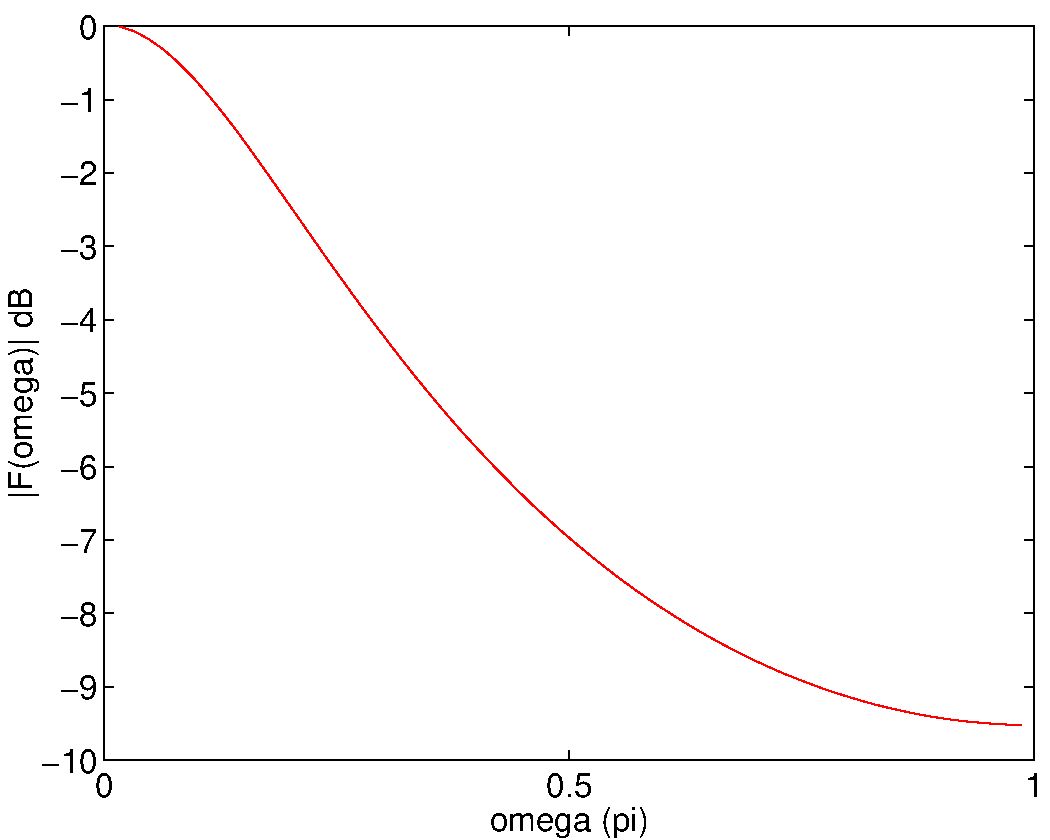
\includegraphics[width=2.5in]{ch-conv/zt_expo_r0-5F}}
\caption{Frequency content of the signal shown
in figure~\protect\ref{fig:zt-expo-r0.5f}.
\label{fig:zt-expo-r0.5F}}
\end{figure}

Figure~\ref{fig:zt-expo-r0.5F} is the plot of
$|\mathcal{X}(\hat{\omega})|$ versus frequency $\omega$.  The
amplitude decreases along increasing frequency. Its peak is at zero
frequency, which is called \emph{DC} (which literally means ``direct
current,'' implying the constant --- actually mean --- component of
the signal).

\paragraph*{When $\alpha=1$:}

For $\alpha=1$, the sequence becomes
\begin{equation}
x[n] = u[n] = \left\{\begin{array}{ll}
                        1 & n \ge 0 \\
                        0 & n < 0
          \end{array}\right.
\end{equation}
or
\begin{equation}
u[n] = \{1, 1, 1, \ldots\}, \quad k \ge 0
\end{equation}

\index{unit step}
This is a discrete time, infinite duration \emph{unit step}
signal. Notice the difference between the unit step signal and the
unit impulse signal. The latter only has one nonzero value at one
particular time, the former has value one for all time after some
particular time. By analogy with $\delta[n]$ , a unit step occurring at
sample $k$ is called $u[n-k]$.  Substituting $\alpha=1$
into~(\ref{eq:zt-expoF}) we have
\index{z-transform!of a unit step}
\begin{equation}
U(z)=\frac{1}{1-z^{-1}}, \quad |z|>1
\end{equation}
We can see that the pole (a zero in the denominator; you'll learn more
about this in Chapter~\ref{ch:fb-filters}) is at $z=1$, where the
z-transform has an infinite value.

Let's evaluate the frequency content of the unit step signal. If we
evaluate $\mathcal{U}(\hat{\omega})$ on the unit circle (except at
$z=1$), we obtain
\begin{align}
\mathcal{U}(\hat{\omega})
&= U(e^{j\hat{\omega}})
  =\frac{1}{1-e^{-j\hat{\omega}}}\frac{e^{j\hat{\omega}/2}}{e^{j\hat{\omega}/2}}
\notag\\
&= \frac{e^{j\hat{\omega}/2}}{e^{j\hat{\omega}/2}-e^{-j\hat{\omega}/2}} \notag\\
&= \frac{e^{j\hat{\omega}/2}}{2j\sin\hat{\omega}/2} \notag\\
&= \frac{e^{j(\hat{\omega}/2-\pi/2)}}{2\sin\hat{\omega}/2}, \quad \hat{\omega}\ne
2\pi k, k=0,1,\ldots
\end{align}
because $-j=e^{-j\pi/2}$ (see the self-test exercises).  Hence, the
presence of a pole (a zero in the denominator) at $z=1$ (that is, at
$\hat{\omega}=0$) creates a problem only when we want to compute
$|\mathcal{U}(\hat{\omega})|$ at $\hat{\omega}=0$, because
$|\mathcal{U}(\hat{\omega})|\rightarrow \infty$ as
$\hat{\omega}\rightarrow 0$. For any other value of $\hat{\omega}$,
$|\mathcal{U}(\hat{\omega})|$ is finite.

\begin{figure}
\centerline{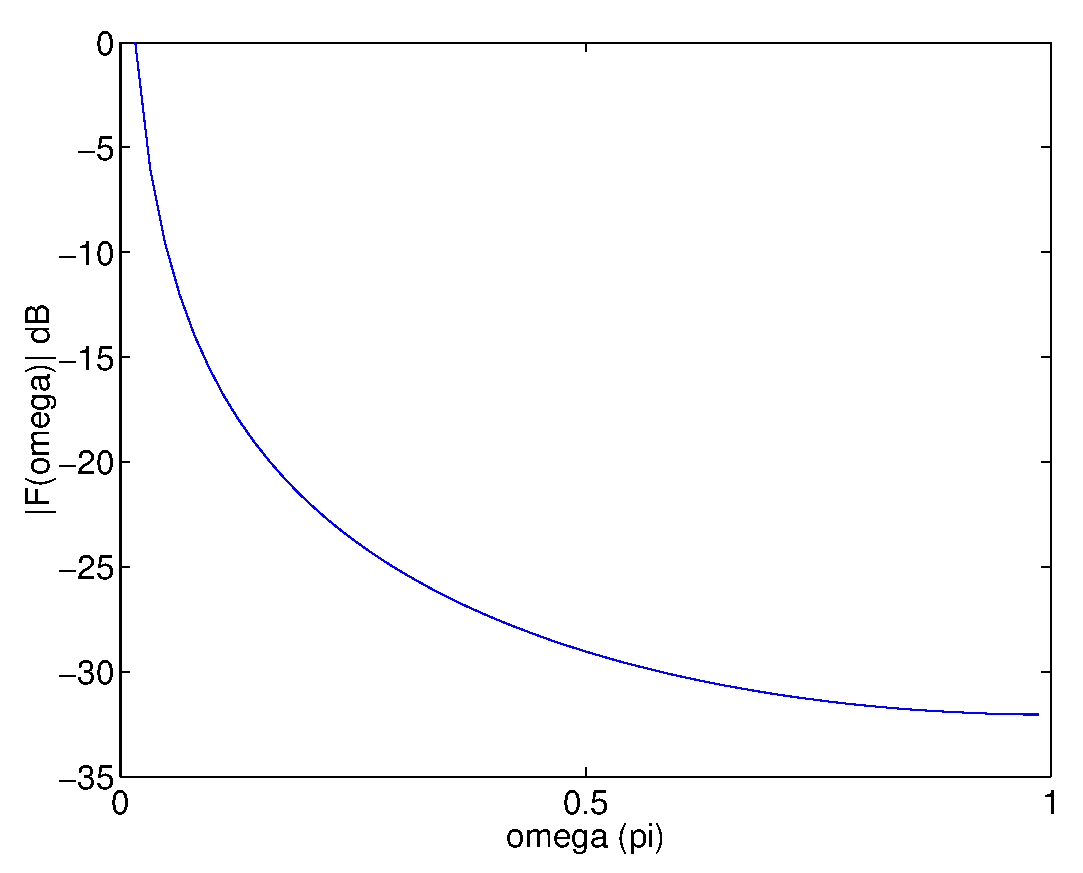
\includegraphics[width=3.5in]{ch-conv/zt_expo_r1F}}
\caption{Frequency content of the unit step signal.
\label{fig:zt-expo-r1F}}
\end{figure}

Figure~\ref{fig:zt-expo-r1F} shows a plot of
$|\mathcal{U}(\hat{\omega})|$ vs.  $\hat{\omega}$.  Since the signal
is a unit step, and so has a constant value from zero onwards, we
might expect the signal to have zero frequency components at all
frequencies except at $\hat{\omega}=0$, but that is not the case. The
reason is that the signal is not a constant for all $-\infty <n<
\infty$. Instead, it is turned on at $n=0$. This \emph{abrupt jump}
creates all the frequency components existing in the range
$0<\hat{\omega}\le\pi$. Generally, \emph{all} signals which start at a
finite time will have nonzero frequency components everywhere in the
frequency axis from zero up to the Nyquist frequency. All such signals
can be considered to be the product of some infinite signal with a
unit step; we will see the effect of this on their spectrum when we
explore convolution in section~\ref{sc:convolution}.

\paragraph*{\textsc{Optional:} When $\alpha$ is a complex number, $\alpha=Re^{j\theta}$:}

When $\alpha=Re^{j\theta}$, equations~(\ref{eq:zt-expof})
and~(\ref{eq:zt-expoF}) become
\begin{equation}
x[n] = \left\{\begin{array}{ll}
                        R^ke^{jn\theta} & \quad  n \ge 0 \\
                        0             & \quad n < 0
          \end{array}\right.
\end{equation}

\begin{equation}
X(z)=\frac{1}{1-Re^{j\theta}z^{-1}}, \quad |z|>|R|
\label{eq:zt-expo-cF}
\end{equation}

When $z=Re^{j\theta}$ we have what we call a \emph{pole} (a zero in the
denominator; you'll learn more about this in
Chapter~\ref{ch:fb-filters}). Equation~(\ref{eq:zt-expo-cF}) can be
broken into real and imaginary parts using Euler's formula:
\begin{align}
X(z) &= \frac{1}{1-Re^{j\theta}z^{-1}} \notag\\
     &= \frac{1}{1-R(\cos\theta+j \sin\theta )z^{-1}} \notag\\
     &= \frac{1}{1-R\cos\theta z^{-1}-j R\sin\theta z^{-1}} \notag\\
     &= \frac{1-R\cos\theta z^{-1}+j R\sin\theta z^{-1}}
     {[1-R\cos\theta z^{-1}]^2 - [jR\sin\theta z^{-1}]^2} \notag\\
     &= \frac{1-R\cos\theta z^{-1}+j R\sin\theta z^{-1}}
     {1-2R\cos\theta z^{-1} + R^2 z^{-2}} \notag\\
     &= \frac{1-R\cos\theta z^{-1}}
     {1-2R\cos\theta z^{-1} + R^2 z^{-2}}
     +j\frac{R\sin\theta z^{-1}}
     {1-2R\cos\theta z^{-1} + R^2 z^{-2}}
\end{align}

We break the signal into two parts, too:
\begin{align}
\Real\{x[n]\} &= R^n\cos(k\theta), \quad n\ge 0\\
\Imag\{x[n]\} &= R^n\sin(k\theta), \quad n\ge 0
\end{align}
From real part we get
\begin{equation}
R^n\cos(n\theta)\stackrel{\mathbf{Z}}{\longleftrightarrow} \
\frac{1-R\cos\theta z^{-1}}
{1-2R\cos\theta z^{-1} + R^2 z^{-2}}
\end{equation}
and from imaginary parts we have
\begin{equation}
R^n\sin(n\theta)\stackrel{\mathbf{Z}}{\longleftrightarrow} \
\frac{R\sin\theta z^{-1}}
{1-2R\cos\theta z^{-1} + R^2 z^{-2}}
\end{equation}

When $R<1$, $R^n\cos(n\theta)$ and $R^n\sin(n\theta)$ are damped
cosine and sine waves.

\problemset{
\subsubsection{Self-Test Exercises}

See~\ref{sc:ch6ex} \#\ref{it:ch6ex5}--\ref{it:ch6ex7} for answers.

\begin{enumerate}
\item What is the derivative of $u[n-k]$ (the unit step at time step
  $k$)?
\item Show that $e^{j\hat{\omega}/2}-e^{-j\hat{\omega}/2} =
  2j\sin\hat{\omega}/2$.
\item Prove that $e^{-j\pi/2}=-j$.
\end{enumerate}}

\section{Convolution}
\label{sc:convolution}

\index{convolution!discrete!definition} Convolution is an important
operation for implementing digital filters.  Let's first define what
convolution is. For two infinite, discrete signals $x[n]$ and $h[n]$,
the \emph{convolution} $y[n]$ of them at sample $n$ is defined as
\begin{equation}
y[n] = \sum_{k=-\infty}^{\infty} h[k] x[n-k]
\label{eq:convolution}
\end{equation}
The notation for convolution is ``$\ast$'', so this can be written as 
\begin{equation}
Y = X \ast H
\end{equation}
where $Y$, $X$, and $H$ are the signals with samples at $n$ being
$y[n]$, $x[n]$, and $h[n]$.

Let's consider the case when both $x$ and $h$ both start at zero. This
is equivalent to saying that both have values of zero before that
sample. So, $h[k] = 0$ when $k<0$ and $x[n-k]=0$ when
$n-k<0$. Equation~(\ref{eq:convolution}) becomes
\begin{equation}
y[n] = \sum_{k=0}^{n} h[k] x[n-k]
\label{eq:zt-conv}
\end{equation}
Actually, this is a more realistic situation than $k$'s summation
from $-\infty$ to $\infty$.

We expand the summation in~(\ref{eq:zt-conv}) as
\begin{multline}
y[n] = h[0] x[n] + h[1] x[n-1] + h[2] x[n-2] + \ldots + h[k] x[n-k]
       + \ldots \\
       {}+ h[n-2] x[2] + h[n-1] x[1] + h[n] x[0]
\label{eq:zt-conv-exp}
\end{multline}
Using this formulation, you may show that the convolution $X \ast H$ has the
following properties:
\begin{enumerate}
\item Commutative: $X \ast H=H \ast X$
\index{convolution!commutative property}
\item Distributive :  $X \ast (H_1 + H_2)=X \ast H_1 + X \ast H_2$
\index{convolution!distributive property}
\item Associative : $(X \ast H) \ast G = X \ast (H \ast G)$
\index{convolution!associative property}
\end{enumerate}
You should be able to convince yourself that $x \ast \vec{0} = \vec{0}
\ast x = 0$ (where $\vec{0}$ is a vector of all zeros). How about
$\vec{1} \ast \vec{1}$ (where $\vec{1}$ is a vector of all ones, in
this case $\vec{1}=u[n]$; see the self-test exercise)?

\subsection{Example of Convolution}

Determine the convolution $e^n \ast e^n$, $n=0,1,2,\ldots,
$. Using~(\ref{eq:zt-conv}),
\begin{align}
e^n \ast e^n &= \sum_{k=0}^{n}e^ke^{n-k} \notag\\
             &= \sum_{k=0}^{n}e^n=e^n\sum_{k=0}^{n}1=ne^n
\end{align}

\problemset{
\subsubsection{Self-Test Exercises}

See~\ref{sc:ch6ex} \#\ref{it:ch6ex8}--\ref{it:ch6ex9} for answers.

\begin{enumerate}
\item Determine if $u[n] \ast H \ne H$ is true, where $h[n] = n$,
$n=0,1,2,\ldots$ (a \emph{ramp}).
\item Compute $u[n] \ast u[n]$.
\end{enumerate}}

\subsection{Implementing Convolution}

\index{convolution!discrete!implementation}
From observation of equation~(\ref{eq:zt-conv-exp}), we know that for
a fixed sample $n$, $y[n]$ can be computed by the term-by-term
multiplication of the sequence
\begin{equation}
\{h[0], h[1], h[2], \ldots, h[k], \ldots, h[n-2], h[n-1], h[n]\}
\end{equation}
and the time-reversed sequence
\begin{equation}
\{x[n], x[n-1], x[n-2], \ldots, x[n-k] , \ldots, x[2], x[1], x[0]\}
\end{equation}
We just multiply the corresponding terms (for example, $h[k]x[n-k]$),
then add these products. This produces the convolution for one sample
$n$.  Remember, however, that the output $y[n]$ is also a sequence,
$n=0,1,2,\ldots$. We need to repeat this process for all $\{n\}$ to
get the full sequence, as shown in algorithm~\ref{alg:convolution}.
 
\begin{algorithm}
\caption{Discrete convolution.\label{alg:convolution}}
\begin{algorithmic}
\REQUIRE $h[n]$ is a finite, discrete signal, $n = 0, 1, 2, \ldots$
\REQUIRE $x[n]$ is a finite, discrete signal, $n = 0, 1, 2, \ldots$
\ENSURE $y[n]$ is the convolution $X * H$, $n = 0, 1, 2, \ldots$
\FOR{$n=0, 1, 2, \ldots$}
   \STATE Reverse $x[k]$ to produce $x'[k] = x[n-k]$, $k = 0, 1, 2,
          \ldots, n$
   \STATE $s[k] = h[k] x'[k]$
   \STATE $y[n] = \sum_{k=0}^n s[k]$
\ENDFOR
\end{algorithmic}
\end{algorithm}

A more-or-less direct implementation of this algorithm in C is:

\index{C code!convolution|(}
\begin{small}
\begin{verbatim}
/* Convolution of two vectors

   Input: vectors x and h of lengths nx and nh (nh < nx)
   Output: vector y of length nx + nh - 1 (storage already allocated)
 */
void convolve(int x[], unsigned nx, int h[], unsigned nh, int y[])
{
   for (unsigned n=0; n<nx+nh-1; n++) {
      y[n] = 0;
      for (unsigned k=max(0,n-nh+1); k<=min(nx-1,n); k++)
         y[n] += x[k] * h[n-k];
   }
}
\end{verbatim}
\end{small}
\index{C code!convolution|)}

\begin{figure}
\centerline{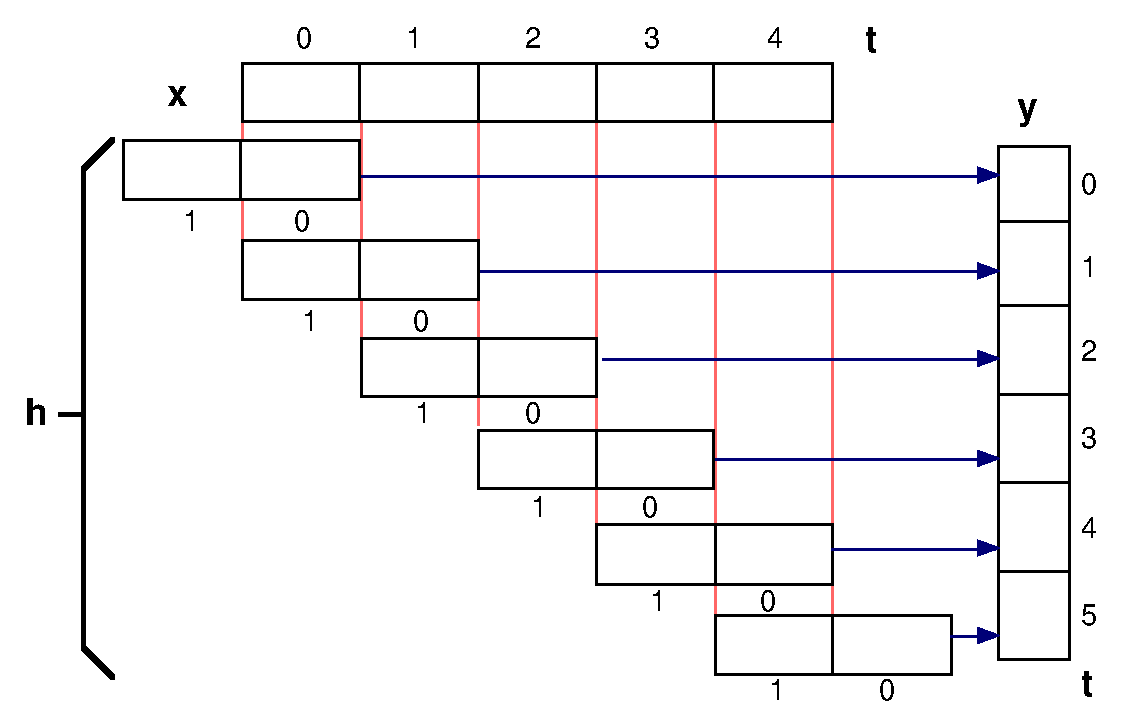
\includegraphics[width=\textwidth]{ch-conv/fig6-5}}
\caption{Example of convolution function execution for $n_x=5$ and
$n_h=2$.\label{fg:convex}}
\end{figure}

You'll notice something nasty was done here: the identities of
$x$ and $h$ were reversed! Of course, this is perfectly OK, given the commutative
property of convolution. This was done because we generally assume that $h$
(the shorter vector) is a property of the filter (we will see about
this later) and it is easier to think about reversing
it than reversing the signal $x$. If for no other reason, this makes
sense because $h$ has a shorter length.

The implementation is for finite-length signals, rather than the
infinite ones we've been discussing. It assumes that $h$ is shorter
than $x$ ($n_h < n_x$). This $h$ input is often called the convolution
\emph{kernel} because, as we shall see, $h$ represents the
\index{convolution!kernel}
action of our signal processing system while $x$ is the actual input
signal.  Notice that, for small $n<n_h-1$, not all of $h$ is
used. This is equivalent to multiplying the unused elements of $h$
against the zero values of $x[k]$, $k<0$. Similarly, for large
$n>nx-1$, part of $h$ is also unused --- multiplied against the zero
values of $x[k]$, $k>n_x-1$. Figure~\ref{fg:convex} illustrates
function execution for a signal $X$ of length 5 and a kernel $H$ of
length 2. This is one way to deal with the \emph{boundary conditions}
\index{convolution!boundary conditions}
associated with the convolution: what to do at the ends of the
signal $X$.  In general, there are three ways of dealing with these
boundary conditions:
\begin{enumerate}
\item ``Pad'' $X$ with zeros past its ends. In effect, this is what
was done in the code above.
\item ``Reflect'' $X$ by copying element $k$ to index $-k$. This is
sometimes done in image processing operations.
\item ``Truncate'' the convolution at the ends of $X$. This means that
$n$ would cover the range $n_h-1 \leq n \leq n_x$ and $Y$ would be
shorter than $X$.
\end{enumerate}

\index{MATLAB code!convolution}
MATLAB has the built-in convolution function \verb|conv|, which takes
two vectors as inputs and outputs the convolution result with length
equal to one less than the sum of the two input vector lengths. You
can use ``\verb|help conv|'' to get more information (how does
\verb|conv| deal with boundary conditions [answer in~\ref{sc:ch6ex}
\#\ref{it:ch6ex10}]?)

\begin{figure}
\centerline{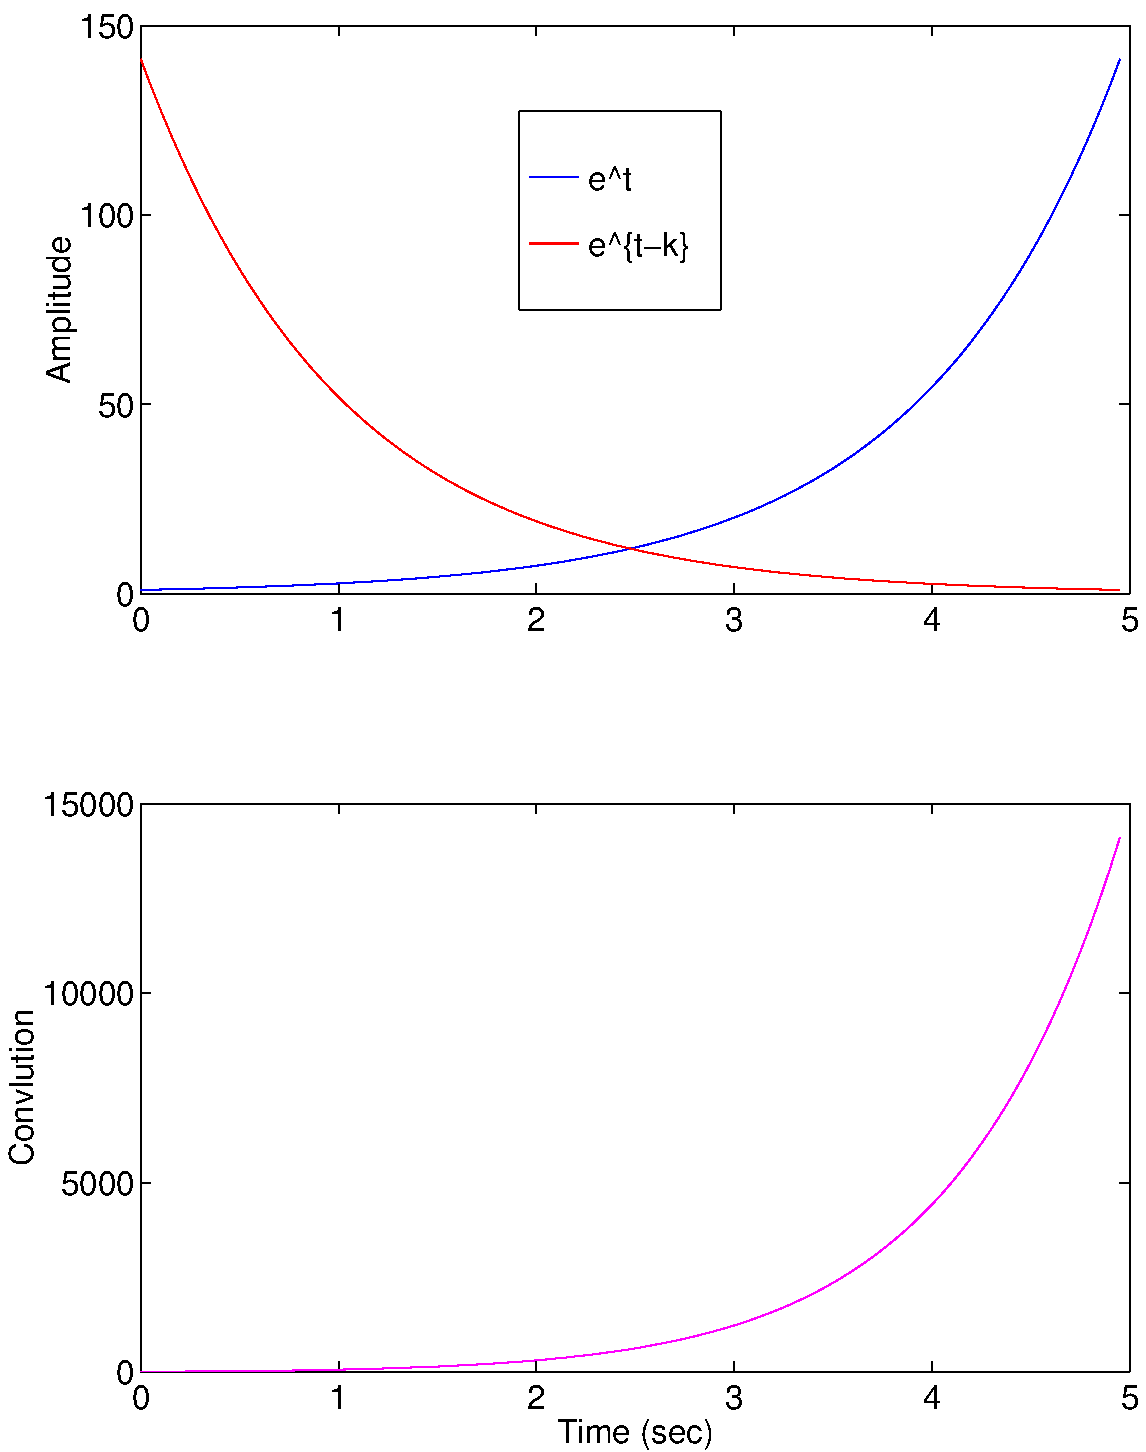
\includegraphics[width=4in]{ch-conv/zt_conv_etet}}
\caption[Convolution of $e^n \ast e^n$]{Convolution of $e^n \ast
  e^n$. Top blue line is $e^n$, top red line is time reversed version
  of $e^n$, the bottom plot is the result of convolution.
  \label{fig:zt-conv-etet}}
\end{figure}

Let's look at the convolution of $X \ast H =e^n \ast e^n$ again. In
this case, $X$ and $H$ are the same function. In
figure~\ref{fig:zt-conv-etet} (top), $X$ is shown as a blue curve and
the time-reversed $H$ is shown as a red curve. The convolution result
is in the bottom graph.

\problemset{
\subsubsection{Self-Test Exercises}

See~\ref{sc:ch6ex} \#\ref{it:ch6ex11} for the answer.

\begin{enumerate}
\item Use MATLAB to compute the convolution $e^{-n}*e^{-n}$ and plot
the result.
\end{enumerate}}

\section{Properties of the Z-Transform}

\index{z-transform!properties of}
\begin{table}
\caption{Some properties of the z-transform.\label{tb:zt-property}}
\begin{center}
\begin{tabular}{|l|c|c|} \hline
Property      & Time Domain, $Z^{-1}\{\cdot\}$ & z-Domain, $Z\{\cdot\}$ \\ \hline\hline
Linearity     & $a_1x[n]+a_2y[n]$ & $a_1X(z)+a_2Y(z)$\\ 
Time shift    & $x[n-k]$       & $z^{-k}X(z)$\\ 
Scaling in the z-domain 
              & $a^nx[n]$        & $X(a^{-1}z)$ \\ 
Time reversal & $x[-n]$        & $X(z^{-1})$\\ 
Differentiation in the z-domain 
              & $nx[n]$          & $-z \deriv{X(z)}{z}$ \\ 
Convolution   & $x[n] \ast y[n]$       & $X(z)Y(z)$ \\ \hline
\end{tabular}
\end{center}
\end{table}

The z-transform is a very powerful signal processing tool because it
has some very important properties. Some of these properties are
listed in
table~\ref{tb:zt-property}, where the time-domain signals $x[k]$
and $y[k]$ have z-transforms of $X(z)$ and $Y(z)$.

Knowing these properties can be very convenient. For example, the
z-transform of a signal shifted (delayed) by $k$ samples, $x[n-k]$,
is $z^{-k}X(z)$; this is our familiar $z$ (delay) operator. You can
\index{z-transform!relation to $z$ operator}
\index{z-transform!and delay}
also see that the convolution property of the z-transform means that
convolution in the time domain is multiplication in the z-domain. So,
if we have the z-transform of two signals, it is much easier to
perform convolution.  Later on, you will find out that this is very
important in filtering. Let's prove this property:

From~(\ref{eq:zt-conv}) a convolution of $x[n]$ and $h[n]$ is defined as:
\begin{equation}
y[n] = x[n] \ast h[n] = \sum_{k=-\infty}^{\infty} h[k] x[n-k]
\end{equation}
The z-transform of $y[n]$ is 
\begin{align}
Y(z) &= \sum_{n=-\infty}^{\infty} y[n]z^{-n} \notag\\
     &= \sum_{n=-\infty}^{\infty}
     \left( \sum_{k=-\infty}^{\infty} h[k] x[n-k] \right)z^{-n}
\end{align}
Interchanging the order of the summations (which is equivalent to
factoring out the $h[k]$ and distributing the $z^{-n}$ over the inner
summation),
\begin{equation}
Y(z) = \sum_{k=-\infty}^{\infty} h[k]
             \left( \sum_{n=-\infty}^{\infty} x[n-k] z^{-n} \right)
\end{equation}
The inner summation is merely the z-transform of $x[n]$ shifted by $k$
samples.  Applying the time shift property of the z-transform, we
obtain
\begin{align}
Y(z) &= \sum_{k=-\infty}^{\infty} h[k] X(z) z^{-k} \notag\\
     &= X(z)\sum_{k=-\infty}^{\infty} h[k] z^{-k} 
     = X(z) H(z)
\end{align}
Which is the product of the two z-transforms. I'll present a couple
examples of using these properties.

\subsection{Example: Time Shifting}

\index{z-transform!of a time-shifted impulse}
Remember that the z-transform of the unit impulse
$\delta[n]$ was previously discussed
\begin{equation}
\delta[n] = \left\{\begin{array}{ll}
                        1 & n=0 \\
                        0 & n \neq 0
          \end{array}\right.
\end{equation}
is 1 and that the z-transform of the shifted unit impulse
$\delta[n-k]$ is $z^{-k}$? Using the time-shifting property of the
z-transform, this is easy to determine:
\begin{equation}
\delta[n]\stackrel{\mathbf{Z}}{\longleftrightarrow} 1
\end{equation}
then 
\begin{equation}
\delta[n-k]\stackrel{\mathbf{Z}}{\longleftrightarrow} 1 \times z^{-k}=z^{-k}
\end{equation}

\subsection{Example: Convolution}

\index{z-transform!computing convolution with}
Given the signals 
\begin{equation}
x[n] = \{1, -3, 2, 1\}, \quad n = 0,1,2,3
\end{equation}
and 
\begin{equation}
h[n] = \left\{\begin{array}{ll}
                        1 &  n=0,1\\
                        0 &  n=2,3
          \end{array}\right.
\end{equation}
use the z-transform to compute their convolution $Y = X \ast H$.

According to~(\ref{eq:zt}),
\begin{align}
X(z) &= 1-3z^{-1}+2z^{-2}+z^{-3}\\
H(z) &= 1+z^{-1}
\end{align}
Then using the convolution property of the z-transform, we have 
\begin{align}
Y(z)=X(z)H(z)
&= (1-3z^{-1}+2z^{-2}+z^{-3})(1+z^{-1}) \notag\\
&= 1-2z^{-1}-z^{-2}+3z^{-3}+z^{-4}
\end{align}
Now we can easily get the inverse z-transform $y[n]=x[n] \ast h[n]$ from the
result $Y(z)$. Again from the z-transform
definition~(\ref{eq:zt}),
\begin{equation}
y[n] = x[n] \ast h[n] = \{1,-2, -1, 3, 1\}
\end{equation}

We can also compute the convolution directly, according to the
convolution definition~(\ref{eq:zt-conv}). There are only 4 nonzero
terms in $x[n]$ and 2 in $h[n]$. For a fixed sample $n$, the
convolution is given by
\begin{align}
y[n] &= \sum_{k=0}^{n} x[k] h[n-k] \notag\\
     &= x[0] h[n] + x[1] h[n-1] + x[2] h[n-2] + x[3] h[n-3]
\end{align}
Changing $n$ gives the sequence of the convolution output as a
function of time. In the following computation, $h[n-k]=0$ is used,
if $n-k<0$ and $x[k]=0$ and $h[k]=0$ if $k>3$:
\begin{align*}
y[0] &= x[0] h[0] = 1\\
y[1] &= x[0] h[1] + x[1] h[0] = 1-3 = -2\\
y[2] &= x[0] h[2] + x[1] h[1] + x[2] h[0] = 0-3+2 = -1\\
y[3] &= x[0] h[3] + x[1] h[2] + x[2] h[1] +x[3] h[0] = 0+0+2+1 = 3\\
y[4] &= x[1] h[3] + x[2] h[2] + x[3] h[1] = 0+0+1 = 1\\
y[n] &= 0, \quad n>4
\end{align*}
Therefore, this also gives the result
\begin{equation}
y[n] = x[n] \ast h[n] = \{1,-2, -1, 3, 1\}
\end{equation}

\problemset{
\subsubsection{Self-Test Exercises}

See~\ref{sc:ch6ex} \#\ref{it:ch6ex12} for the answer.

\begin{enumerate}
\item Prove the scaling property of the z-transform; that is, if 
  \begin{equation*}
    x[n]\stackrel{\mathbf{Z}}{\longleftrightarrow} X(z)
  \end{equation*}
  then 
  \begin{equation*}
    a^n x[n]\stackrel{\mathbf{Z}}{\longleftrightarrow} X(a^{-1}z)
  \end{equation*}
\end{enumerate}}

\section{Impulse Response and the Transfer Function}

Recall the a filter's input/output relationship is summarized by the
transfer function discussed in chapter~\ref{ch:filt-intro} (and which
you'll see again in chapter~\ref{ch:fb-filters}). Let's denote the
input signal as $x[n]$ and output as $y[n]$ in the time domain. You
learned that the the transfer function in the z domain is $H(z)$. What
is its time domain representation? We will answer this shortly; first
let's give a name to the time domain transfer function,
$h[n]$: the filter's
\emph{impulse response}. The filter's input/output relationship can be
\index{filter!impulse response}
written using $h[n]$ as:
\begin{equation}
y[n] = x[n] \ast h[n]
\label{eq:zt-hx}
\end{equation}
This says that the output of filter results from the convolution
between input signal $x[n]$ and filter's impulse response $h[n]$. From
earlier in this chapter, you now know that convolution of two signals
in the time domain is equivalent to multiplying their z-transforms in
the $z$ domain. So, we obtain the input/output relationship via the
transfer function in the $z$ domain as
\begin{equation}
Y(z) =X(z)H(z)
\label{eq:zt-HX}
\end{equation}
where $X(z)$ and $Y(z)$ are the z-transforms of $x[n]$ and $y[n]$ and
$H(z)$ is the z-transform of $h[n]$.  Actually, this $H(z)$ is just
the transfer function we talked about in chapter~\ref{ch:filt-intro}.
In other words, a filter's transfer function is the z-transform of its
impulse response!
\index{z-transform!relationship to filter transfer function}
\index{filter!transfer function!relationship to its z-transform}

\index{filter!transfer function!determining with z-transform}
As a simple example of how to use the z-transform to determine a
filter's transfer function from its defining equation, consider the
feedforward filter:
\begin{equation}
y[n] = b_0x[n] + b_1x[n-k]
\end{equation}

Applying the z-transform to both sides, 
\begin{equation}
Y(z) = b_0X(z) + b_1z^{-k}X(z)
\end{equation}
because of the time shift property of the z-transform. This can be
rearranged to be
\begin{equation}
Y(z) = (b_0 + b_1z^{-k})X(z)
\end{equation}
So the transfer function is 
\begin{equation}
H(z) = b_0 + b_1z^{-k}
\end{equation}
and therefore, we have
\begin{equation}
Y(z)=H(z)X(z)
\end{equation} 

Applying the inverse z-transform, we can get the time domain
representation of $H(z)$, or the impulse response $h[n]$. In a similar
manner, we can get the output $y[n]$ from $Y(z)$.  In fact,
using~(\ref{eq:zt-HX}), we found an easy way to compute a filter's
response to a signal if we have already know the signal's z-transform
and the filter's transfer function.

Let's see why $h[n]$ is called the impulse response.  Remember the unit
impulse, which is a signal that has the value one at $n=0$ and zero
otherwise, and which can be expressed as
\begin{equation}
\delta[n] = \left\{\begin{array}{ll}
                        1 & n=0 \\
                        0 & n \neq 0
          \end{array}\right.
\end{equation}

The impulse response of a filter is its output when a unit impulse is
applied. Now we compute these two functions' convolution,
\begin{equation}
y[n]=\sum_{k=0}^{n}\delta[k] h[n-k] = h[n]
\end{equation}
because all of the terms except $k=0$ drop out (since $\delta[k]=0$
for all $k \ne 0$).  This tell us that the filter response $y[n]$ to a
unit impulse is $h[n]$. This is why $h[n]$ is called the impulse
response.

Applying the z-transform to both side of the above equation, we get
\begin{equation}
Y(z)= H(z)
\end{equation}
Therefore, the \emph{transfer function} can be viewed as the
z-transform of the filter's \emph{impulse response}, or its impulse
response in the $z$ domain.

If we restrict $z$ to lie on the unit circle, $z=e^{j\hat{\omega}}$,
from~(\ref{eq:zt-HX}) we obtain
\begin{equation}
\mathcal{Y}(\hat{\omega})=\mathcal{H}(\hat{\omega})\mathcal{X}(\hat{\omega})
\end{equation} 
where $\mathcal{X}(\hat{\omega})$ is the signal's frequency content,
$\mathcal{Y}(\hat{\omega})$ is the frequency content of the filter
output and $\mathcal{H}(\hat{\omega})$ is the filter's frequency
response.


\section{Problems}

\begin{enumerate}
\item Compute the z-transform of 
\begin{equation}
x[n] = \left\{\begin{array}{ll}
                        (-1)^n & n \ge 0 \\
                        0 & n < 0
          \end{array}\right.
\end{equation}
and determine its frequency content. 

\item Determine the z-transform of the signal 
\begin{equation}
x[n] = \left\{\begin{array}{ll}
                        \cos\hat{\omega}_0 n & n \ge 0 \\
                        0 & n < 0
          \end{array}\right.
\end{equation}

\item Find the z-transform of the signal
\[x[n] = \left\{\begin{array}{ll} 1/n! & n \geq 0 \\
                0 & n < 0 \end{array} \right. \]
Recall that $0!=1$.

\item The impulse response of a system is $h[n]=\{1,2,1,-1\}$, $n=-1,
0,1,2$. Determine the response of the system to the input signal
$x[n]=\{1,2,3,1\}$, $n=0, 1,2,3$.

\end{enumerate}


\section{Further Reading}

\begin{itemize}
\item James H McClellan, Ronald W. Schafer, and Mark A. Yoder,
  \textit{DSP First: A Multimedia Approach}, Prentice Hall, 1998,
  chapter 7 (\S 7.1--7.6.3).
\end{itemize}

% LocalWords:  DTFT signal's feedforward
